\documentclass[10pt]{beamer}

\mode<presentation>
{
  \usetheme[height=1.25cm]{Madrid}
  \setbeamertemplate{navigation symbols}{}
  \setbeamercolor{alerted text}{fg=illini}
}

\graphicspath{{figs/}}

\usebackgroundtemplate{
\includegraphics[width=\paperwidth,height=\paperheight]{uc-background}}

\usepackage[english]{babel}
\usepackage{epsfig,subfigure,bm}
\usepackage{multimedia}
\usepackage{psfrag}
\usepackage{animate}

% \usefonttheme{metropolis} % default family is serif
%%%%%% Begin of my macros and options

\setbeamertemplate{section in toc shaded}[default][55]
\setbeamertemplate{subsection in toc shaded}[default][55]
\setbeamercolor{block title}{fg=white,bg=illini}
\setbeamercolor{block body}{fg=black,bg=mygrey}

\setbeamercolor{emphprimary}{fg=CBlue}
\setbeamercolor{emphsecondary}{fg=illini}
\setbeamercolor{emphtertiary}{fg=mygreen}
\definecolor{darkForestGreen}{rgb}{.1,1,.1}
\definecolor{veryLightGray}{rgb}{.9,.9,.9}
\definecolor{greenApple}{rgb}{.3,.9,.3}

\setbeamercolor{title}{bg=CBlue}

\usepackage{amsmath,amssymb,amsxtra,amsthm}
\usepackage{algorithm,algorithmic}
\usepackage{natbib}
\usepackage{bibentry}
\usepackage{xspace}
\usepackage{changepage}

\definecolor{myblue}{rgb}{.2,.2,.7}
\definecolor{myred}{rgb}{.7,.2,.2}
\definecolor{mygreen}{rgb}{.2,.7,.2}
\definecolor{mygrey}{rgb}{0.9,0.9,0.9}
\definecolor{CBlue}{cmyk}{1,0.25,0,0}
\definecolor{illini}{rgb}{0.98,0.4,0.05}
\definecolor{black}{cmyk}{0,0,0,1}

\newcommand{\myemph}[1]{{\usebeamercolor[fg]{emphprimary}
    \textbf{#1}}}
\newcommand{\myemphalt}[1]{{\usebeamercolor[fg]{emphsecondary}
    \textbf{#1}}}

\graphicspath{{figs/}}

\title[Math for Robotics] % (optional, use only with long paper titles)
{CSE276C - Differential Geometry}

\author[H.~I. Christensen] % (optional, use only with lots of authors)
{Henrik I.~Christensen}
% - Give the names in the same order as the appear in the paper.  -
% Use the \inst{?} command only if the authors have different
% affiliation.

\AtBeginSection[]
{
   \begin{frame}
       \frametitle{Outline}
       \tableofcontents[currentsection]
   \end{frame}
}

\institute[UCSD] % (optional, but mostly needed)
{
  \begin{minipage}[c]{.2\textwidth}
    
\includegraphics[width=.65\linewidth]{ucsealnew}%
  \end{minipage}%
  \begin{minipage}[c]{.6\textwidth}
    \small
%%    \begin{center}
      Computer Science and Engineering\\
      University of California, San Diego\\
%%    \end{center}

  \end{minipage}
%%  \vspace*{1ex}
}
%% - Use the \inst command only if there are several affiliations.
%% - Keep it simple, no one is interested in your street address.

\bigskip

\date[Nov 2020]% (optional, should be abbreviation of conference name)
{\small%
  November 2020}

\begin{document}

\nobibliography{/Users/hic/Dropbox/bibliography/bib-file}
\bibliographystyle{plain}

\begin{frame}[plain]
  \titlepage 
\end{frame}

\begin{frame}
  \frametitle{Introduction}
  \begin{itemize}
  \item We can only touch on the basics, but valuable to have basic
    knowledge
  \item Differential Geometry is all about moving on a curve /
    manifold
  \item Robotics is all about moving considering not only kinematics,
    but also dynamics
  \item What motion is possible in a particular space
  \end{itemize}
\end{frame}

\begin{frame}
  \frametitle{Basic Concepts}
  \begin{columns}
    \column{7cm}
    \begin{itemize}
    \item Tangent vector
      \begin{itemize}
      \item A vector anchored at a point p
      \item Set of possible vectors for p is termed tangent space $T_p$
      \end{itemize}
    \end{itemize}
    \column{4cm}
    \vfill
    \centerline{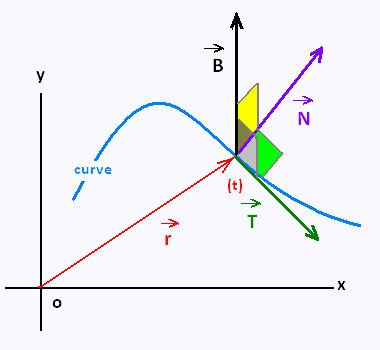
\includegraphics[width=3.8cm]{curve_binormal}}
    \vfill
  \end{columns}
\end{frame}

\begin{frame}
  \frametitle{Basic Concepts}
  \begin{columns}
    \column{7cm}
    \begin{itemize}
    \item Tangent Bundle
      \begin{itemize}
      \item A space along with its tangent vectors
      \item If $\mathbb{R}^n$ the underlying space and we have a
        tangent space of $\mathbb{R}^n$ anchored at each of the
        relevant points
      \item Space is then $\mathbb{R}^n \times \mathbb{R}^n$
      \item So a tangent bundle for a circle would be $S^1 \times \mathbb{R}^1$
      \end{itemize}
    \end{itemize}
    \column{4cm}
    \vfill
    \centerline{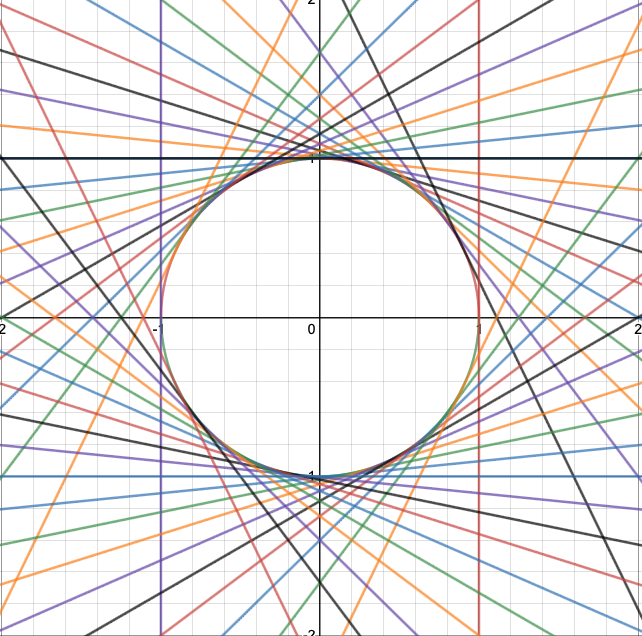
\includegraphics[width=3.8cm]{circle-bundle}}
    \vfill
  \end{columns}
\end{frame}

\begin{frame}
  \frametitle{Basic Concepts}
  \begin{itemize}
  \item Vector Field
    \begin{itemize}
    \item A function that maps a manifold to a tangent space
    \item $M \rightarrow T(M)$ and within it $p \rightarrow v_p \in T_p$ 
    \item Frequently denoted $V(p)$ or $V_p$ 
    \item A classic question: does a manifold has a continuously
      changing vector field that is non-zero?  \pause
    \item The circle example with $M=S^1$ is one such vector field
    \end{itemize}
  \end{itemize}
\end{frame}


\begin{frame}
  \frametitle{Geometry of curves in $\mathbb{R}^3$}
  \begin{itemize}
  \item Consider parameterized curves $\alpha (t) = (x(t), y(t), z(t))$
  \item In general a curve $\alpha$ is a mapping $\alpha: I \rightarrow \mathbb{R}^3$
  \item I is an interval in $\mathbb{R}$ sometimes we will write it as $(\alpha_1 (t), \alpha_2 (t), \alpha_3 (t))$
  \item In general $(x(t), y(t), z(t))$ are differentiable
  \item I.e., has derivatives of all orders throughout I
  \end{itemize}
\end{frame}

\begin{frame}
  \frametitle{A simple 2D example}
  \begin{columns}
    \column{4cm}
    \vfill
    \centerline{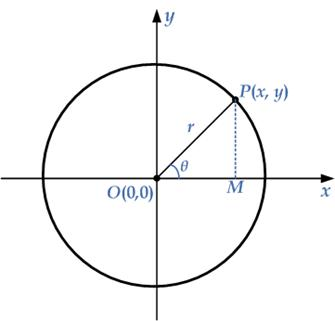
\includegraphics[width=3.8cm]{circle}}
    \vfill
    \column{7cm}
    \begin{itemize}
    \item $\alpha_1 (\theta) = (r \cos (\theta), r \sin (\theta))$
    \item $\theta \in [0, 2 \pi] = I$ OR
    \item $\alpha_2 (\theta) = (r \cos (2 \theta), r \sin (2\theta))$
    \item $\theta \in [0, \pi] = I$ 
    \end{itemize}
  \end{columns}
  \centering
  Different curves / parameterizations can have the same trace
\end{frame}

\begin{frame}
  \frametitle{Simple 3D curve}
  \begin{columns}
    \column{7cm}
    \begin{itemize}
    \item $\alpha (t) = ( a \cos(t), a \sin(t), b t)$, with $ t \in \mathbb{R}$
    \end{itemize}
    \column{4cm}
    \centerline{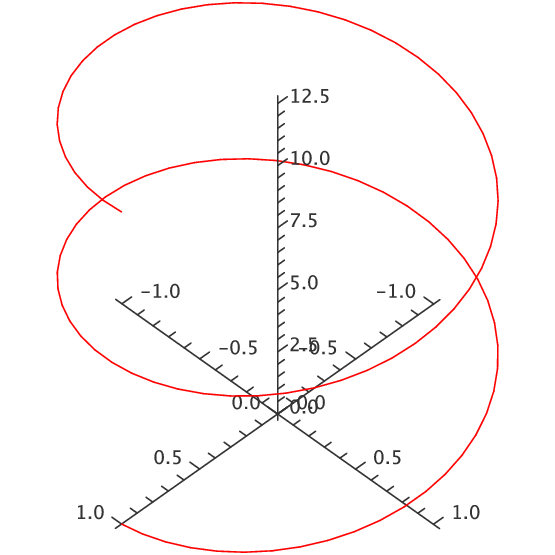
\includegraphics[width=3.8cm]{helix1}}
  \end{columns}
\end{frame}

\begin{frame}
  \frametitle{Velocity vector \& Arclength}
  \begin{itemize}
  \item The velocity vector of $\alpha$ at time t is the vangent vector of $\mathbb{R}^3$ given by
    \[ \alpha'(t) = ( \alpha'_1(t), \alpha'_2(t), \alpha'_3(t)) \]
  \item This vector is obviously also the tangent
  \item The speed of $\alpha$ is $v(t) = ||\alpha'(t)||$
  \item The arclength traversed between $t_0$ and $t_1$ is
    \[
      \int_{t_0}^{t_1} v(t) dt
    \]
  \item You can reparameterize $\alpha (t)$ as $\beta (s)$ where is
    the arclength, which is the same as representing $\alpha$ at unit
    speed
  \end{itemize}
\end{frame}

\begin{frame}
  \frametitle{Simple Example --  Helix}
  \begin{itemize}
  \item Consider the helix: $\alpha(t) = ( r \cos(t), r \sin(t), q t )$ then
    \begin{itemize}
    \item Velocity: $\alpha'(t) = ( - r \sin (t), r \cos (t), q)$
    \item Speed: $ v(t) = \sqrt{ r^2 + q^2 } = c$ a constant
    \item Arclength: $s(t) = \int_0^t c dt = ct$. Thus $t(s) = \frac{s}{c}$
    \item Reparameterized: $\beta(s) = \alpha(\frac{s}{c}) = (r \cos (\frac{s}{c}), r \sin(\frac{s}{c}), q \frac{s}{c})$
    \end{itemize}
  \end{itemize}
\end{frame}

\begin{frame}
  \frametitle{Arclength?}
  \begin{itemize}
  \item So does the integral
    \[
      s(t) = \int_{t_0}^{t_1} ||\alpha'(t)|| dt
    \]
    always converge? \pause
  \item Some curves have infinite arclength (ex fractals - Koch Snowflake) 
    \centerline{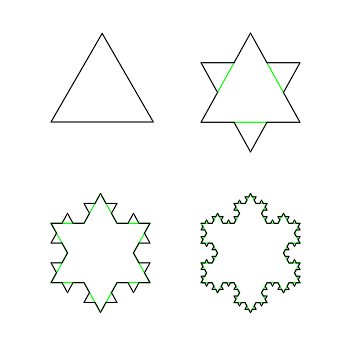
\includegraphics[height=4cm]{koch-flake}}
  \end{itemize}
\end{frame}

\begin{frame}
  \frametitle{Vector fields of $\beta$}
  \begin{itemize}
  \item We can define a set of vector fields for $\beta$
    \begin{itemize}
    \item $T = \beta'$ the unit tangent field
    \item $N = \frac{T'}{||T'||}$ the principal normal vector field
    \item $B = T \times N$ called the binormal vector field of $\beta$
    \end{itemize}
  \item The quantity $||T'||$ is also named the curvature function $K(s) = ||T'(s)||$
  \item The triple (T,N,B) is called the Frenet Frame field of $\beta$
  \end{itemize}
\end{frame}

\begin{frame}
  \frametitle{Curvature}
  \begin{itemize}
  \item Let $\alpha: I \rightarrow \mathbb{R}^3$ be a curve parameterized by arclength
  \item Curvature is then defined as $||\alpha''(s)|| = K(s)$
  \item $\alpha'(s)$ -- the tangent vector of s
  \item $\alpha''(s)$ -- the change in the tangent vector 
  \item $R(s) = 1/K(s)$ -- is called the radius of curvature
  \end{itemize}
\end{frame}

\begin{frame}
  \frametitle{Simple examples}
  \begin{itemize}
  \item Straight line
    \[
      \begin{array}{rcl}
        \alpha(s)   & = & us + v, \mbox{~~~} u,v \in \mathbb{R}^2\\
        \alpha'(s)  & = & u\\
        \alpha''(s) & = & 0 \Rightarrow ||\alpha''(s)|| = 0\\
      \end{array}
    \]
  \item Circle
    \[
      \begin{array}{rcl}
        \alpha(s)   & = & (a \cos (s/a), a \sin (s/a)), \mbox{~~~} s \in [0,2 \pi a]\\
        \alpha'(s)  & = & ( -\sin(s/a), \cos (s/a))\\
        \alpha''(s) & = & (-\cos (s/a) / a, -\sin(s/a) / a) \Rightarrow ||\alpha''(s)|| = 1/a\\
      \end{array}
    \]
  \end{itemize}
\end{frame}

\begin{frame}
  \frametitle{Curvature examples}
  \begin{columns}
    \column{7cm}
    \begin{itemize}
    \item Cornu Spiral - K(s) = s
    \item Generalized Cornu Spirals - K(s) - Polynomial of s
    \end{itemize}
    \column{4cm}
    \centerline{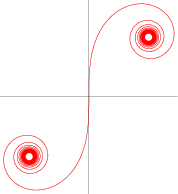
\includegraphics[height=3cm]{CornuSpiral}}
    \centerline{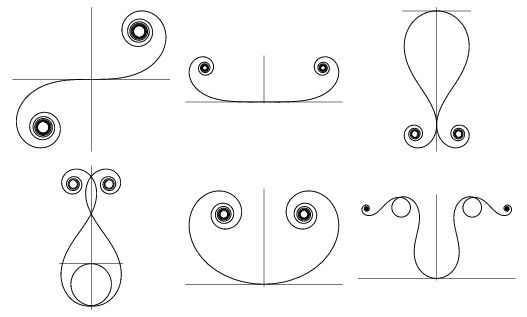
\includegraphics[height=3cm]{CornuPolynomialSpirals}}
  \end{columns}
\end{frame}

\begin{frame}
  \frametitle{Normals}
  \begin{itemize}
  \item When $\alpha$ is parametertized by arc length
    \[
      \alpha'(s) \cdot \alpha'(s) = 1
    \]
  \item From Vector Calculus
    \begin{itemize}
    \item If f, g: $I \rightarrow \mathbb{R}^3$ and $f(t) \cdot  g(t) = const$ for all t
    \item then
      \[ f'(t) \cdot g(t) = -f(t) \cdot g'(t) \] for f * f this is only true for f'(t) f(t) = 0
    \end{itemize}
  \item This implies that
    \[ \alpha''(s) \cdot  alpha'(s) = 0 \]
    or $\alpha''(s)$ is orthogonal to $\alpha'(s)$
  \item Its proportional to the normal of the curve
  \end{itemize}
\end{frame}

\begin{frame}
  \frametitle{Normals}
  \begin{columns}
    \column{7cm}
    \begin{itemize}
    \item $\alpha'(s) = T(s)$ -- Tangent Vector
    \item $||\alpha'(s)||$ -- arc length
    \item $\alpha''(s) = T'(s)$ -- normal direction
    \item $||\alpha''(s)||$ -- curvature
    \item If $||\alpha''(s) \neq 0$ then $\alpha''(s) = T'(s) = K(s) N(s)$
    \end{itemize}
    \column{4cm}
    \vfill
    \centerline{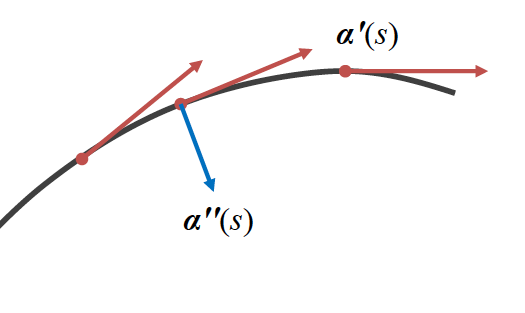
\includegraphics[width=3.8cm]{normals}}
    \vfill
  \end{columns}
\end{frame}

\begin{frame}
  \frametitle{Osculating Plane}
  \begin{columns}
    \column{4cm}
    \vfill
    \centerline{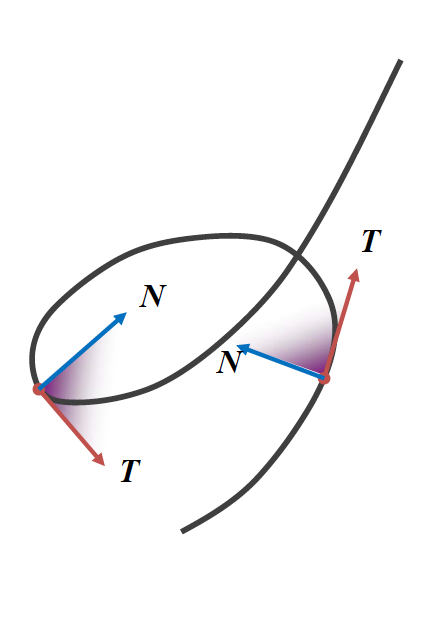
\includegraphics[width=3.5cm]{osculating-plane}}
    \vfill
    Source: M. Ben-Chen, Stanford
    \column{7cm}
    \begin{itemize}
    \item The local plane determined by the unit tangent and the
      normal vectors - T(s) and N(s) is call the osculating plane at s
    \end{itemize}
  \end{columns}
\end{frame}

\begin{frame}
  \frametitle{The Binormal Vector}
  \begin{columns}
    \column{7cm}
    \begin{itemize}
    \item The binormal is defined for $K(s) \neq 0$ by
      \[
        B(s) = T(s) \times N(s)
      \]
    \item The binormal defines the osculating plane
    \end{itemize}
    \column{4cm}
    \vfill
    \centerline{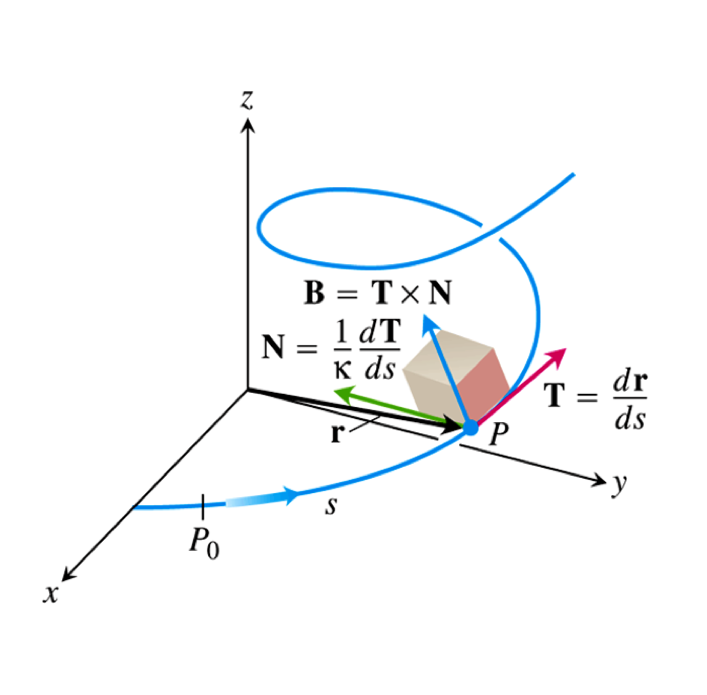
\includegraphics[width=3.5cm]{binormal}}
    \vfill
    Source: R. Gardner, ETSU
  \end{columns}
\end{frame}

\begin{frame}
  \frametitle{The Frenet Frame}
  \begin{columns}
    \column{5cm}
    \vfill
    \centerline{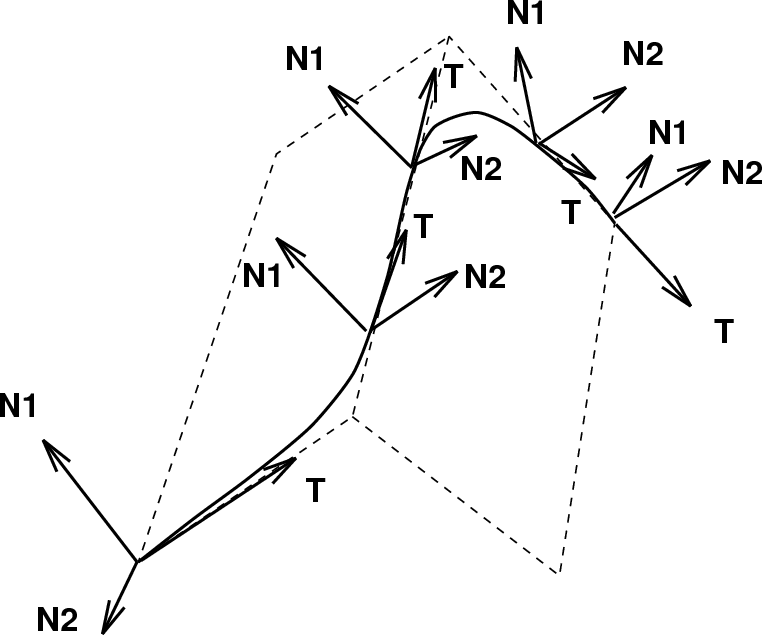
\includegraphics[width=3.8cm]{frenet-frame}}
    \vfill
    Source: A. J. Hanson, LBL
    \column{6cm}
    \begin{itemize}
    \item The system $\{ T(s), N(s), B(s) \}$ for an orthonormal basis for $\mathbb{R}^3$ called the Fernet Frame
    \item The obvious question - How does it change along a curve? I.e., what are T'(s), N'(s), and B'(s)?
    \end{itemize}
  \end{columns}
\end{frame}

\begin{frame}
  \frametitle{T'(s)}
  \begin{itemize}
  \item We have already covered T'(s)
    \[
      T'(s) = K(s) N(s)
    \]

  \item As it is in the direction of N(s) it is orthogonal to B(s) and T(s). 
  \end{itemize}
\end{frame}

\begin{frame}
  \frametitle{N'(s)}
  \begin{itemize}
  \item We know that $N(s) \cdot N(s) = 1$ 
  \item From our earlier lemma (vector calculus) $N'(s) \cdot N(s) = 0$
  \item We know $N(s) \cdot T(s) = 0$ from the lemma $N'(s)\cdot T(s) = -N(s) \cdot T'(s)$
  \item Given $K(s) = N(s) \cdot T'(s)$
  \item It must be true that $N'(s) \cdot T(s) = -K(s)$
  \end{itemize}
\end{frame}

\begin{frame}
  \frametitle{Torsion}
  \begin{itemize}
  \item For the parameterized curve $\alpha: I \rightarrow \mathbb{R}^3$ the torsion of $\alpha$ is defined by
    \[
      \tau(s) = N'(s) \cdot B(s)
    \]
  \item We can then express
    \[
      N'(s) = K(s) T(s) + \tau (s) B(s)
    \]
  \end{itemize}
\end{frame}

\begin{frame}
  \frametitle{Curvature vs Torsion}
  \begin{itemize}
  \item \myemph{Curvature} indicates how much the normal changes in the direction of the tangent
  \item \myemph{Torsion} indicates how much the normal change in the direction orthogonal to the osculating plane
  \item Curvature is always positive, the torsion can be negative
  \item Neither depend on the choice of parameterization 
  \end{itemize}
\end{frame}

\begin{frame}
  \frametitle{B'(s)}
  \begin{itemize}
  \item We know that $B(s) \cdot B(s) = 1$
  \item From the lemma we know $B'(s) \cdot B(s) = 0$
  \item We further know: $B(s) \cdot T(s) = 0$ and $B(s) \cdot N(s) = 0$
  \item From the lemma:
    \[
      B'(s) \cdot T(s) = -B(s) \cdot T'(s) = B(s) \cdot K(s) N(s) = 0
    \]
  \item We get
    \[
      B'(s) \cdot N(s) = -B(s) \cdot N'(s) = - \tau(s)
    \] and from this we have
    \[
      B'(s) = - \tau(s) N(s)
    \]
  \end{itemize}
\end{frame}

\begin{frame}
  \frametitle{The Frenet Formulas}
  \[
    \begin{array}{rclll}
      T'(s)   &=& & K(s) N(s )& \\
      N'(s)   &=&-K(s) T(s) && + \tau(s) B(s)\\
      B'(s)   & =& & -\tau(s) N(s) \\
    \end{array}
  \]
  In Matrix Form
  \[
    \left(
      \begin{array}{ccc}
        | & | & | \\
        T'(s) & N'(s) & B'(s)\\
        | & | & | \\
      \end{array}
    \right) =
    \left(
      \begin{array}{ccc}
        | & | & | \\
        T(s) & N(s) & B(s)\\
        | & | & | \\
      \end{array}
    \right)
    \left(
      \begin{array}{ccc}
        0 & K(s)& 0 \\
        K(s) & 0 & -\tau(s)\\
        0  & \tau(s) & 0\\
      \end{array}
    \right)
  \]
\end{frame}

\begin{frame}
  \frametitle{Example - Back to the helix}
  \begin{itemize}
  \item For: $\alpha(t) = (a \cos(t), a \sin(t), bt)$
  \item Re-paramaterized: $\alpha(s) = (a \cos(s/c), a \sin(s/c), b s/c)$ where $c = \sqrt{a^2 + b^2}$
  \item Curvature is then: $K(s) = \frac{a}{a^2+b^2}$
  \item Torsion is then $\tau(s) = \frac{}{a^2+b^2}$
  \item Note for this example both curvature and torsion are constants
  \end{itemize}
\end{frame}
\end{document}

%%% Local Variables:
%%% mode: latex
%%% TeX-master: t
%%% End:
